\documentclass[logo,reportComp]{thesis}
\usepackage[cpp,pseudo]{mypackage}

\title{计算机图形学}
\subtitle{作业二:Blender图像渲染}
\school{数据科学与计算机学院}
\author{陈鸿峥}
\classname{17大数据与人工智能}
\stunum{17341015}
\headercontext{计算机图形学作业}
\lstset{language=python}

\begin{document}

\maketitle

虽然Blender Beginner Tutoria的视频大约只有5个小时,但我花了至少两倍于它的时间在这上面。
一方面是由于我使用的Blender版本太高(2.8),界面与之前的版本有较大区别,导致花费了大量时间在搜索上面。
另一方面则是视频教程还是略快,up主一直使用快捷键,导致很难跟上他的速度,经常要暂停回放。
而且还不能保证做的方式跟他完全一致,也使得后面的步骤可能会出现一些问题,需要回头重新做过。

但不管怎样,整个学习过程还是很愉悦的。
看见最终渲染出来的结果,十分欣慰,也确实被Blender强大的功能震撼到了。
最终的结果如下图所示。
\begin{figure}[H]
\centering
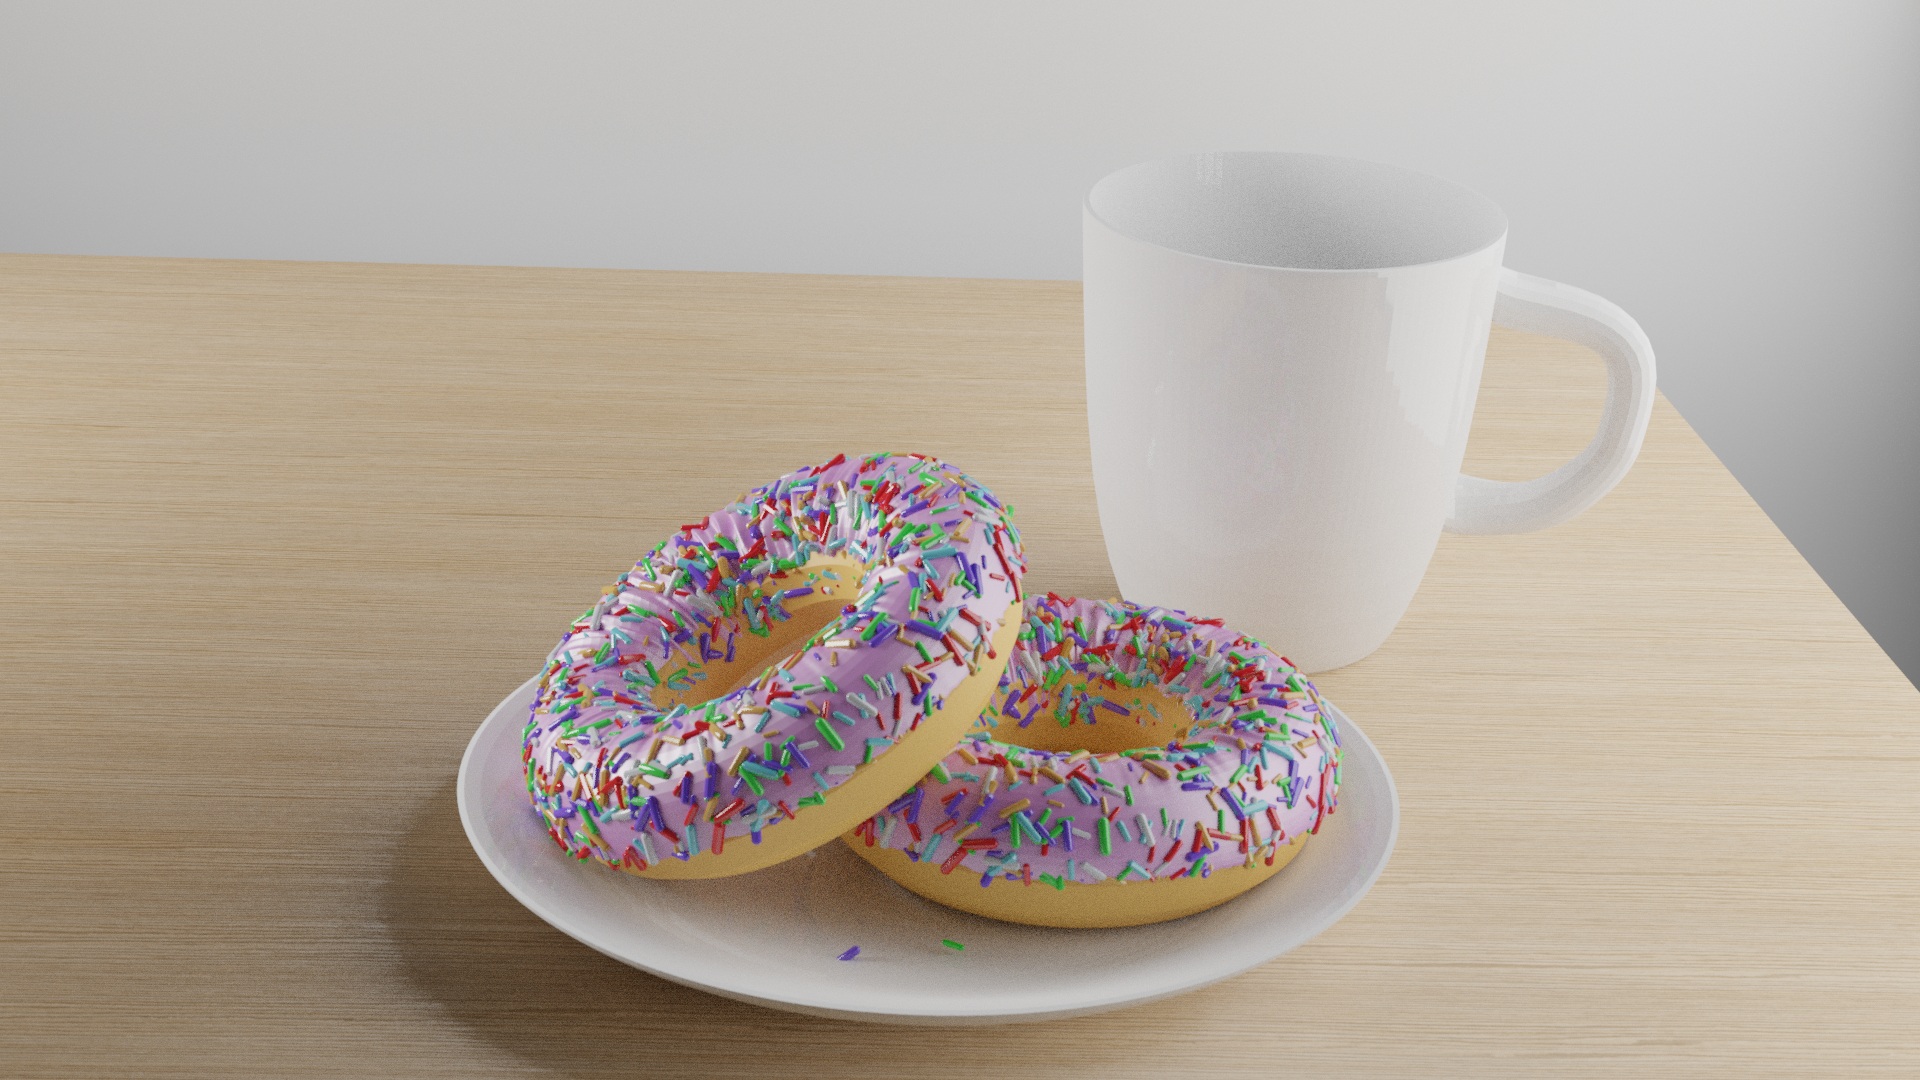
\includegraphics[width=\linewidth]{result.png}
\end{figure}

其他中间过程如下面所示。
\begin{figure}[H]
\centering
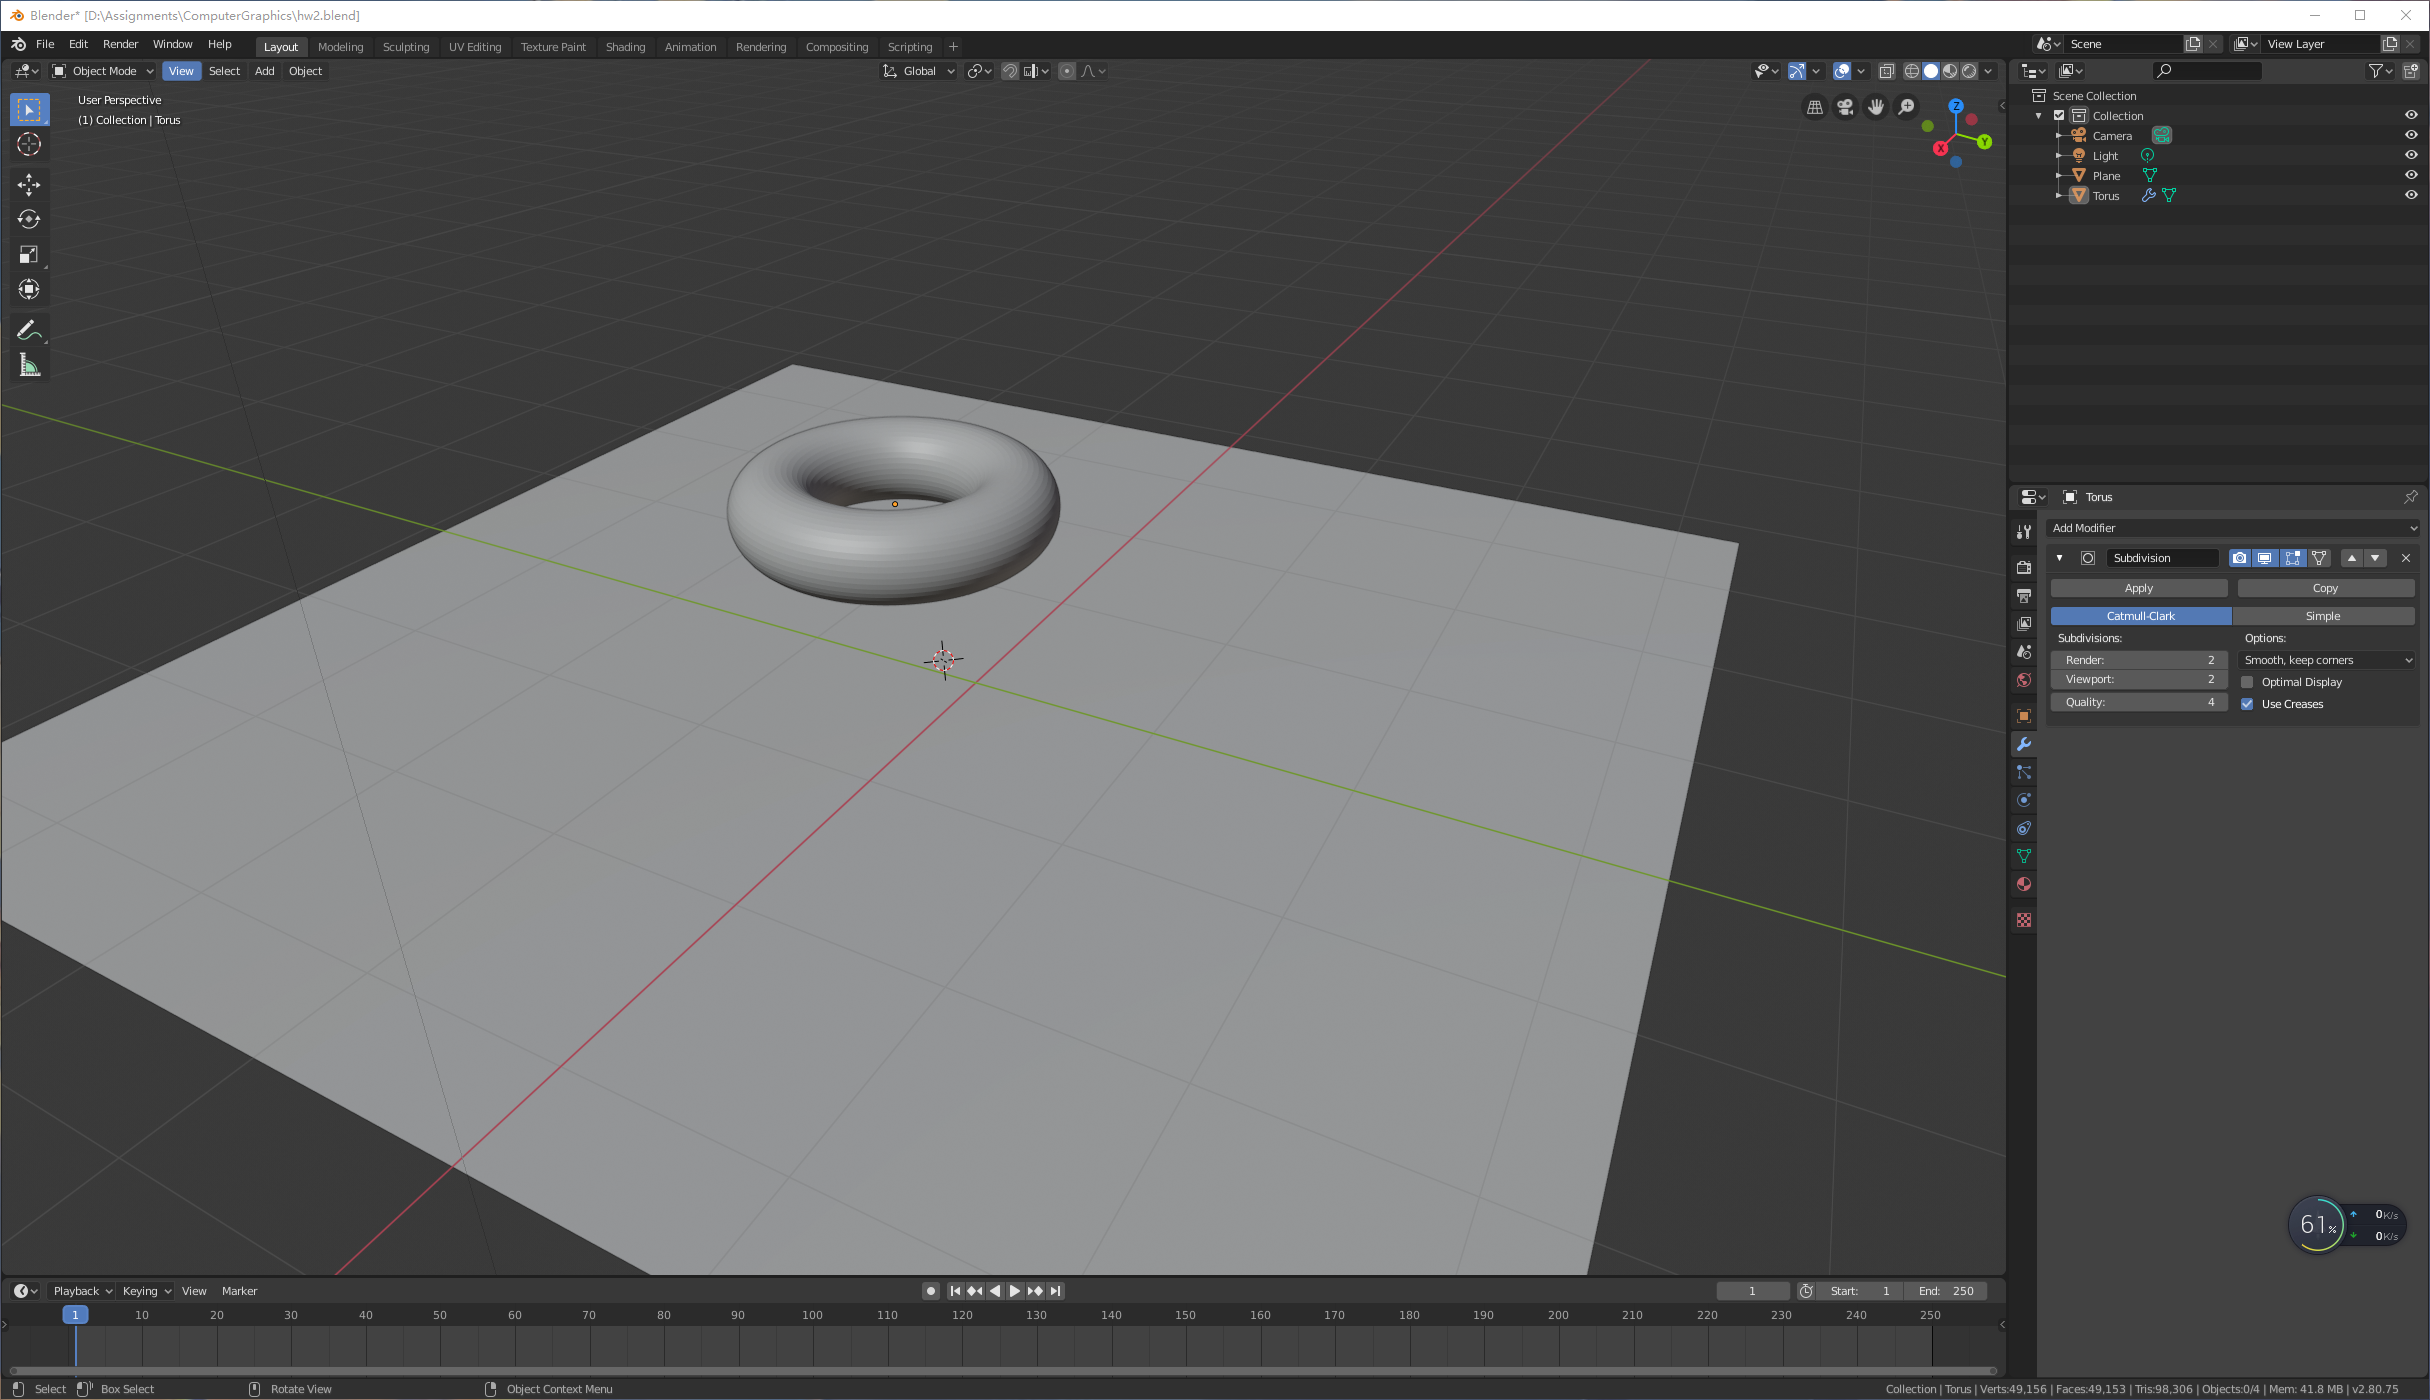
\includegraphics[width=\linewidth]{fig/v2.png}
\end{figure}
\begin{figure}[H]
\centering
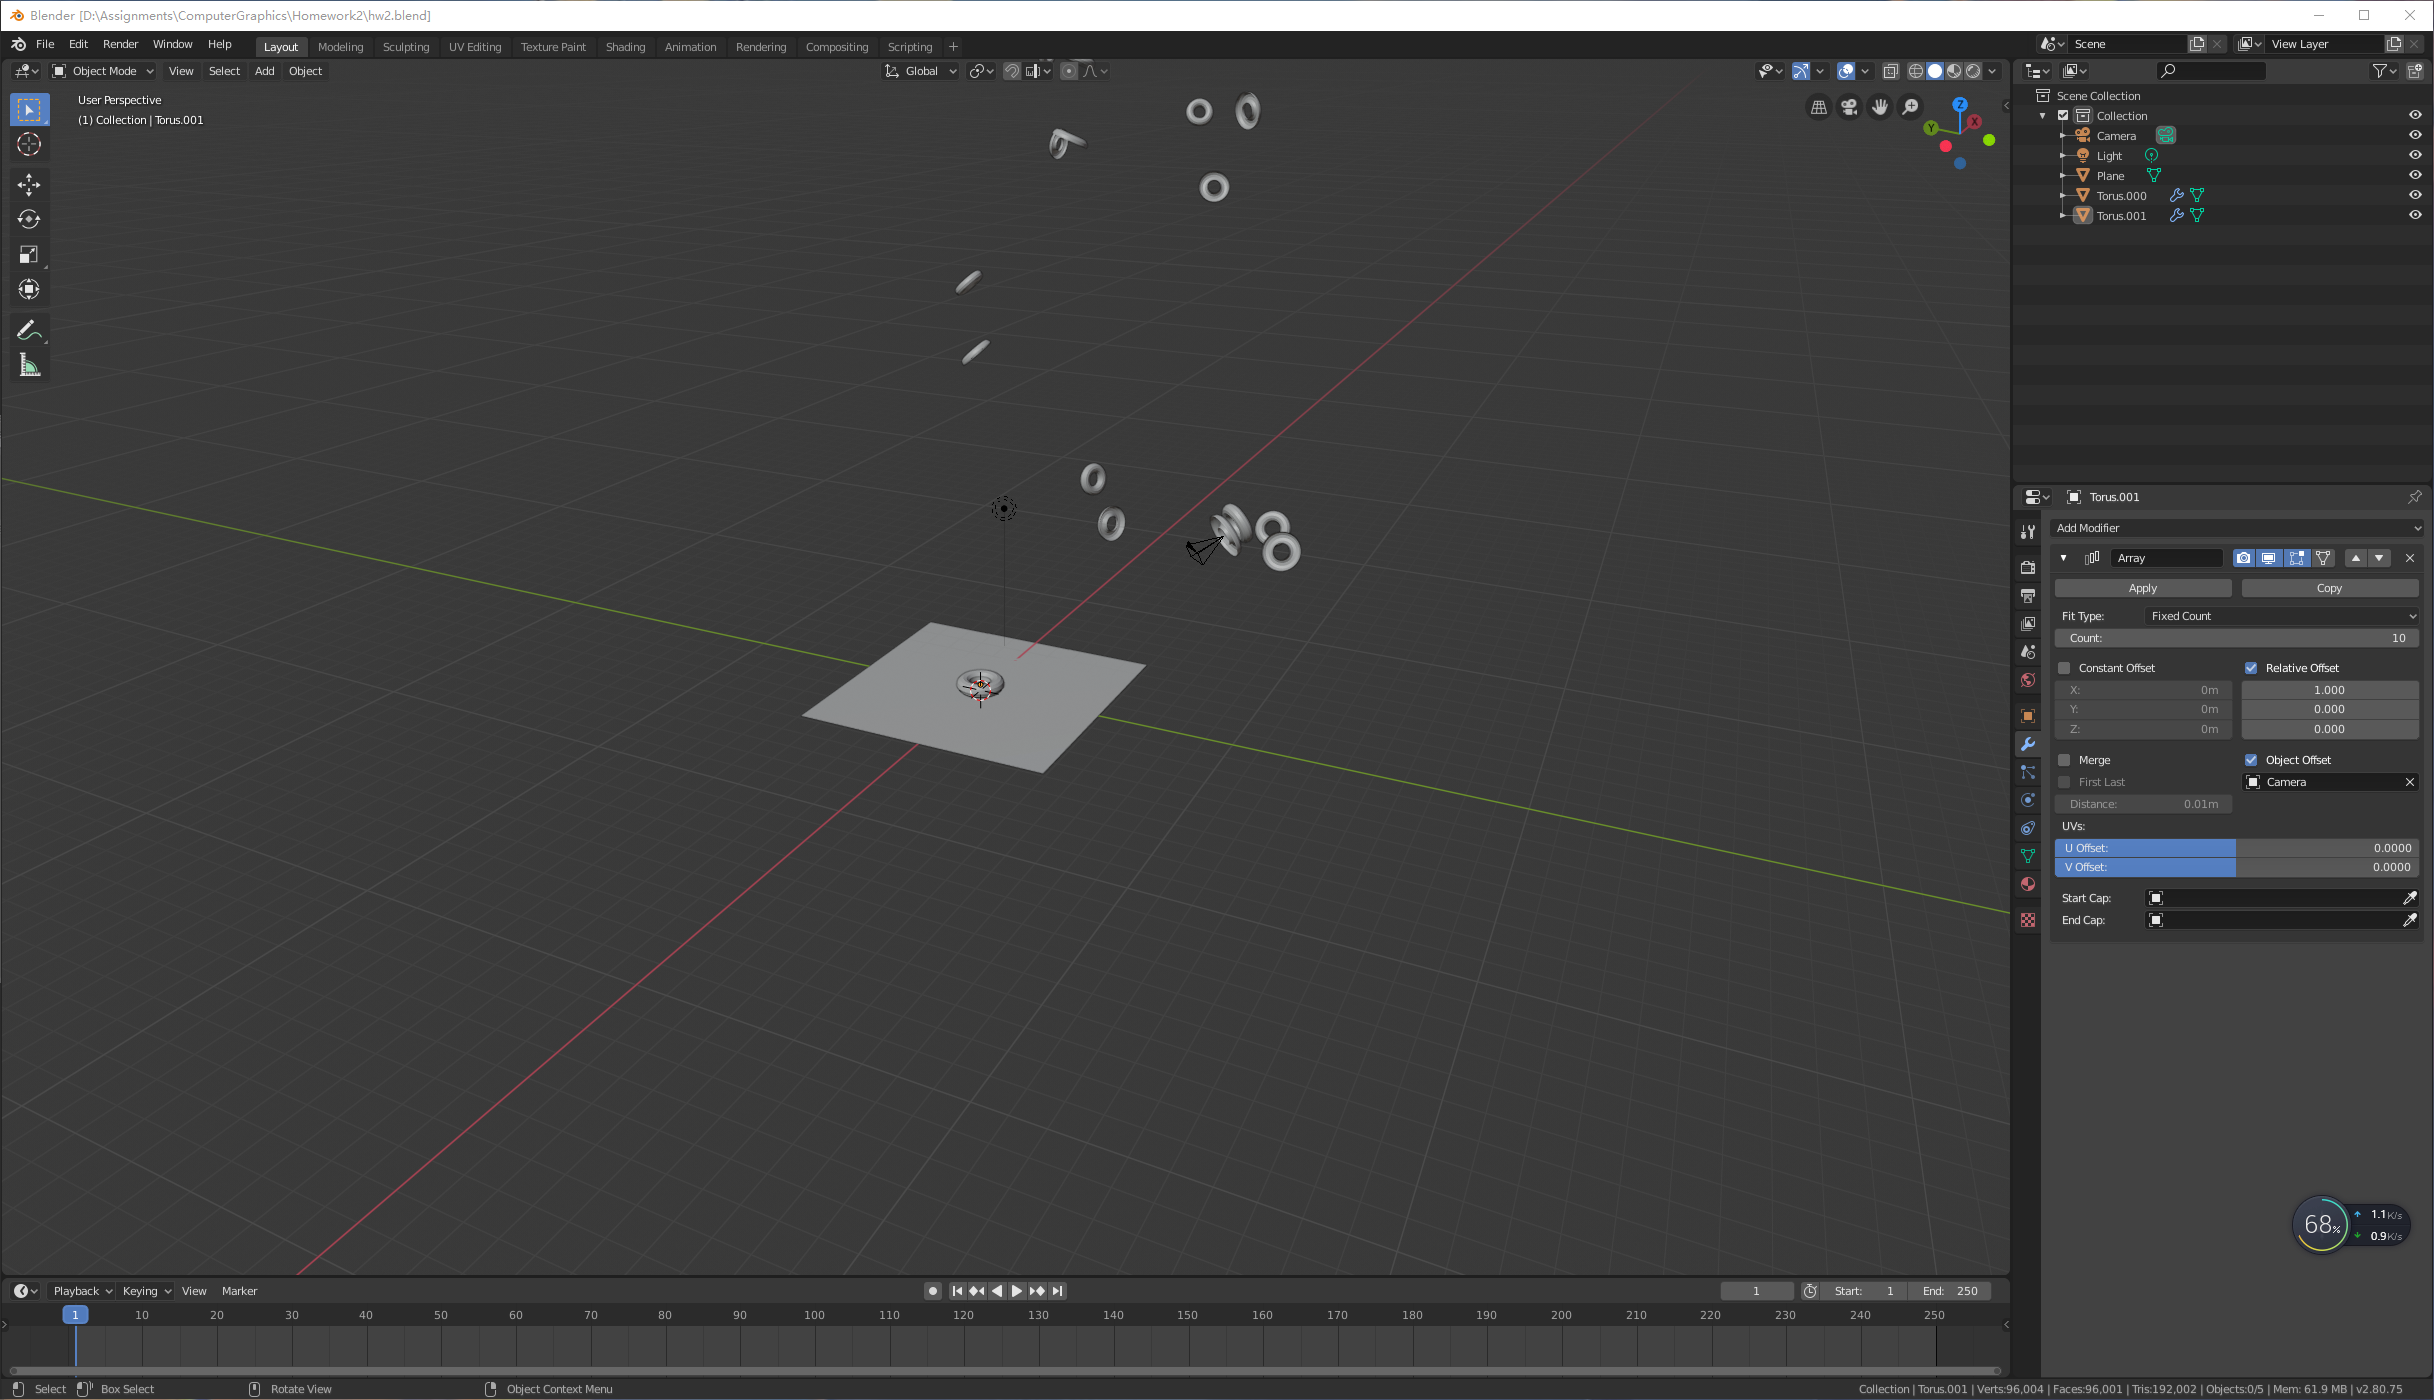
\includegraphics[width=\linewidth]{fig/v3.png}
\end{figure}
\begin{figure}[H]
\centering
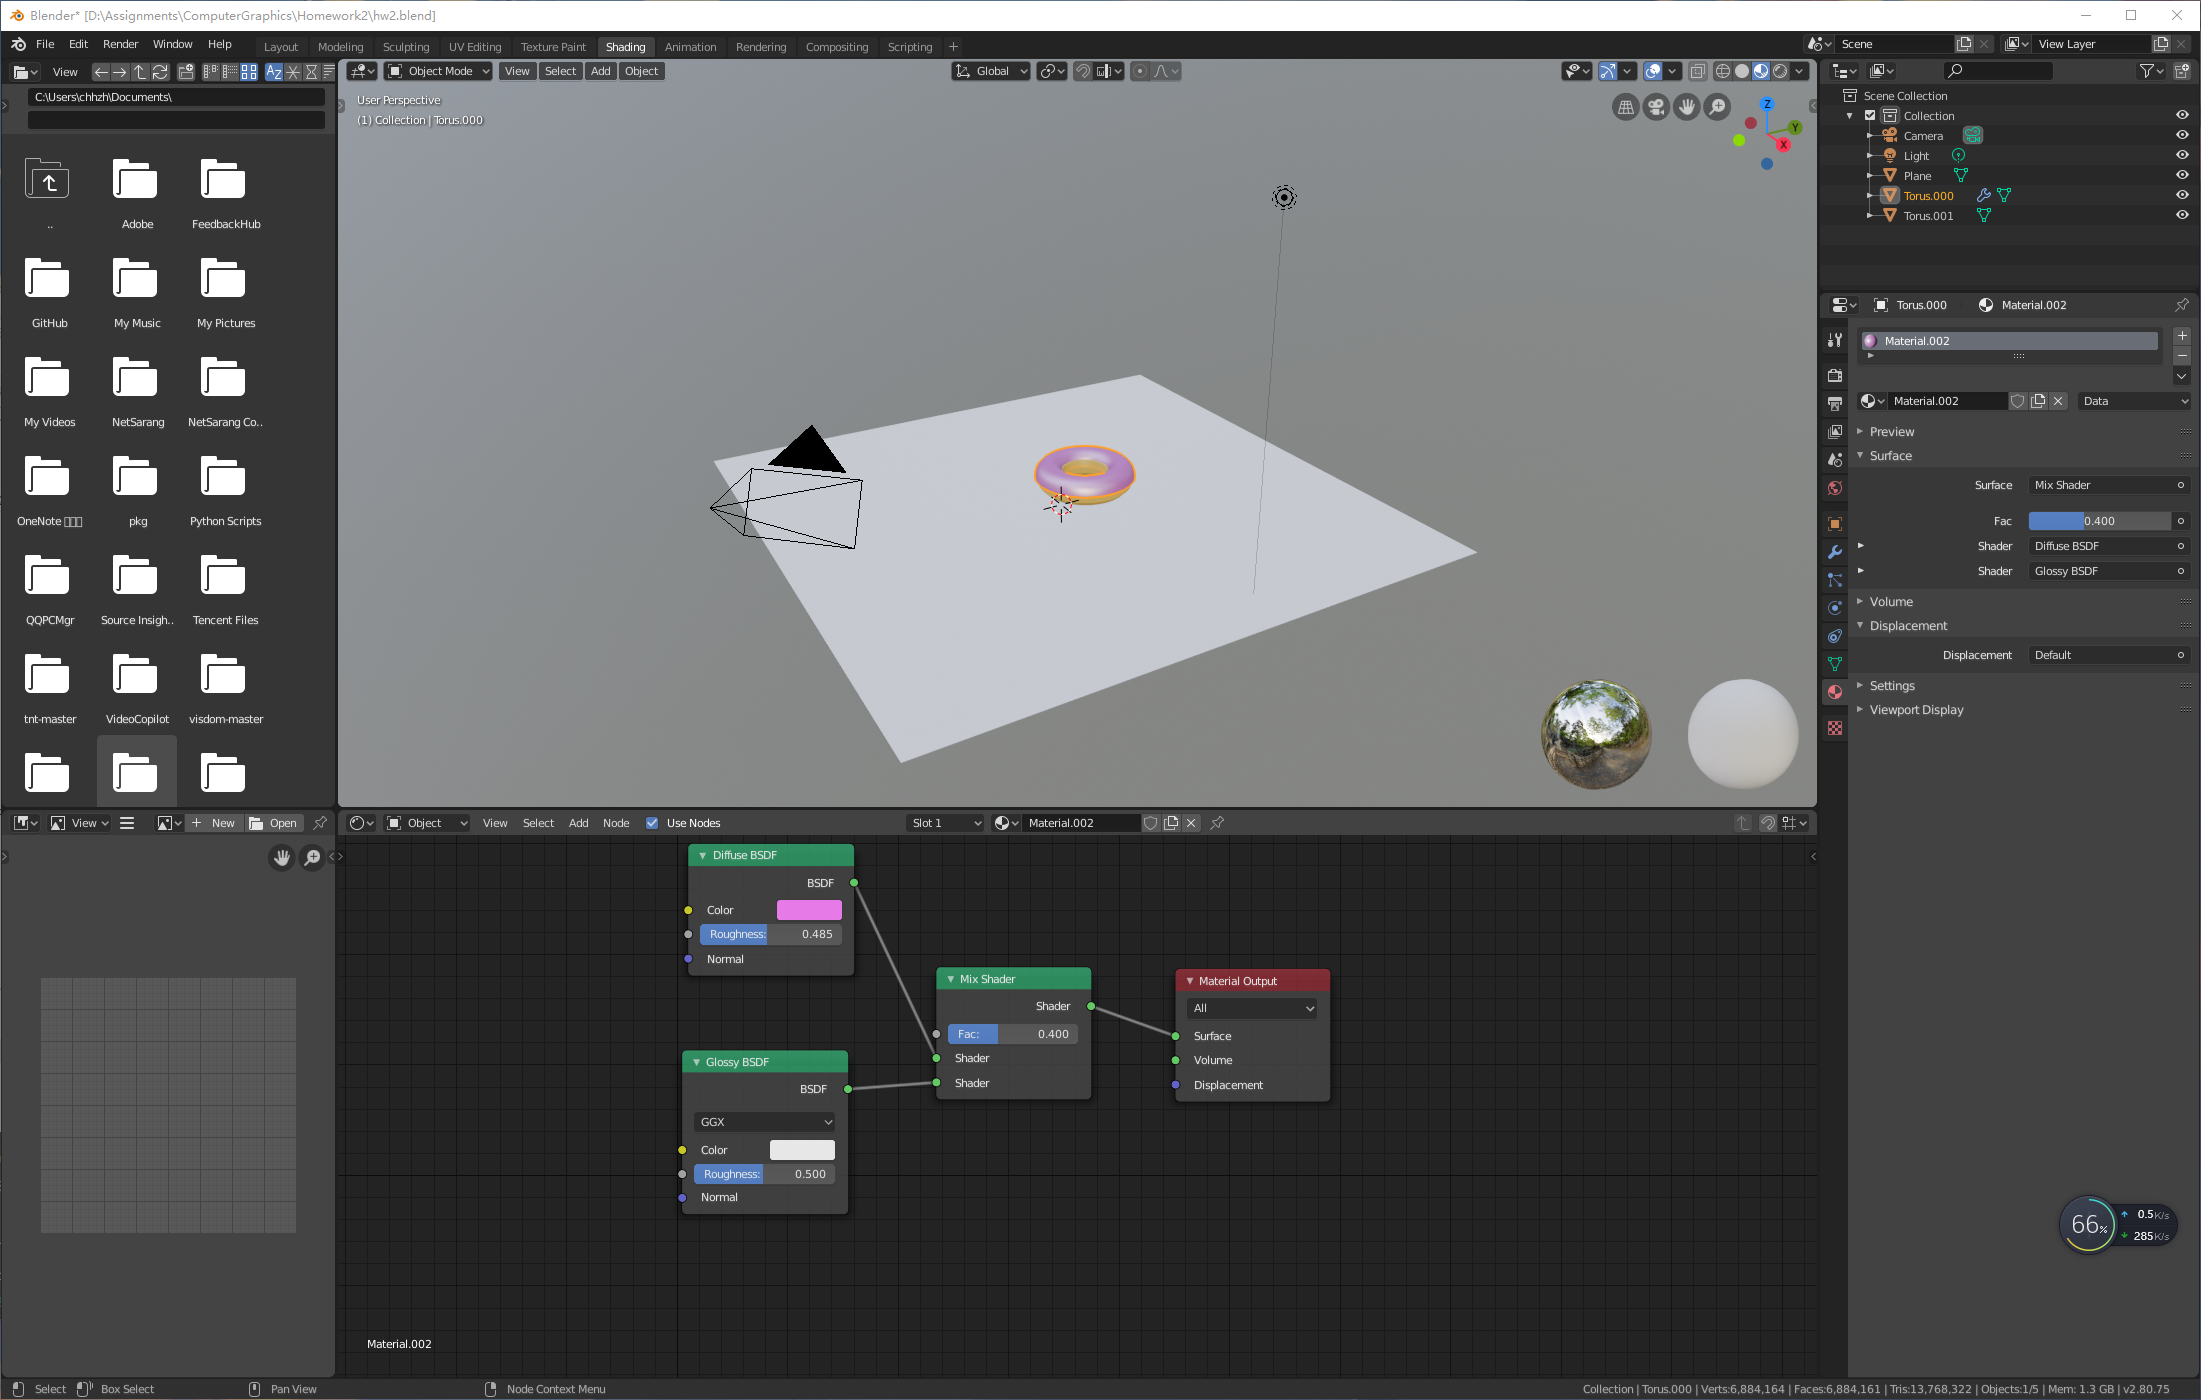
\includegraphics[width=\linewidth]{fig/v4.png}
\end{figure}
\begin{figure}[H]
\centering
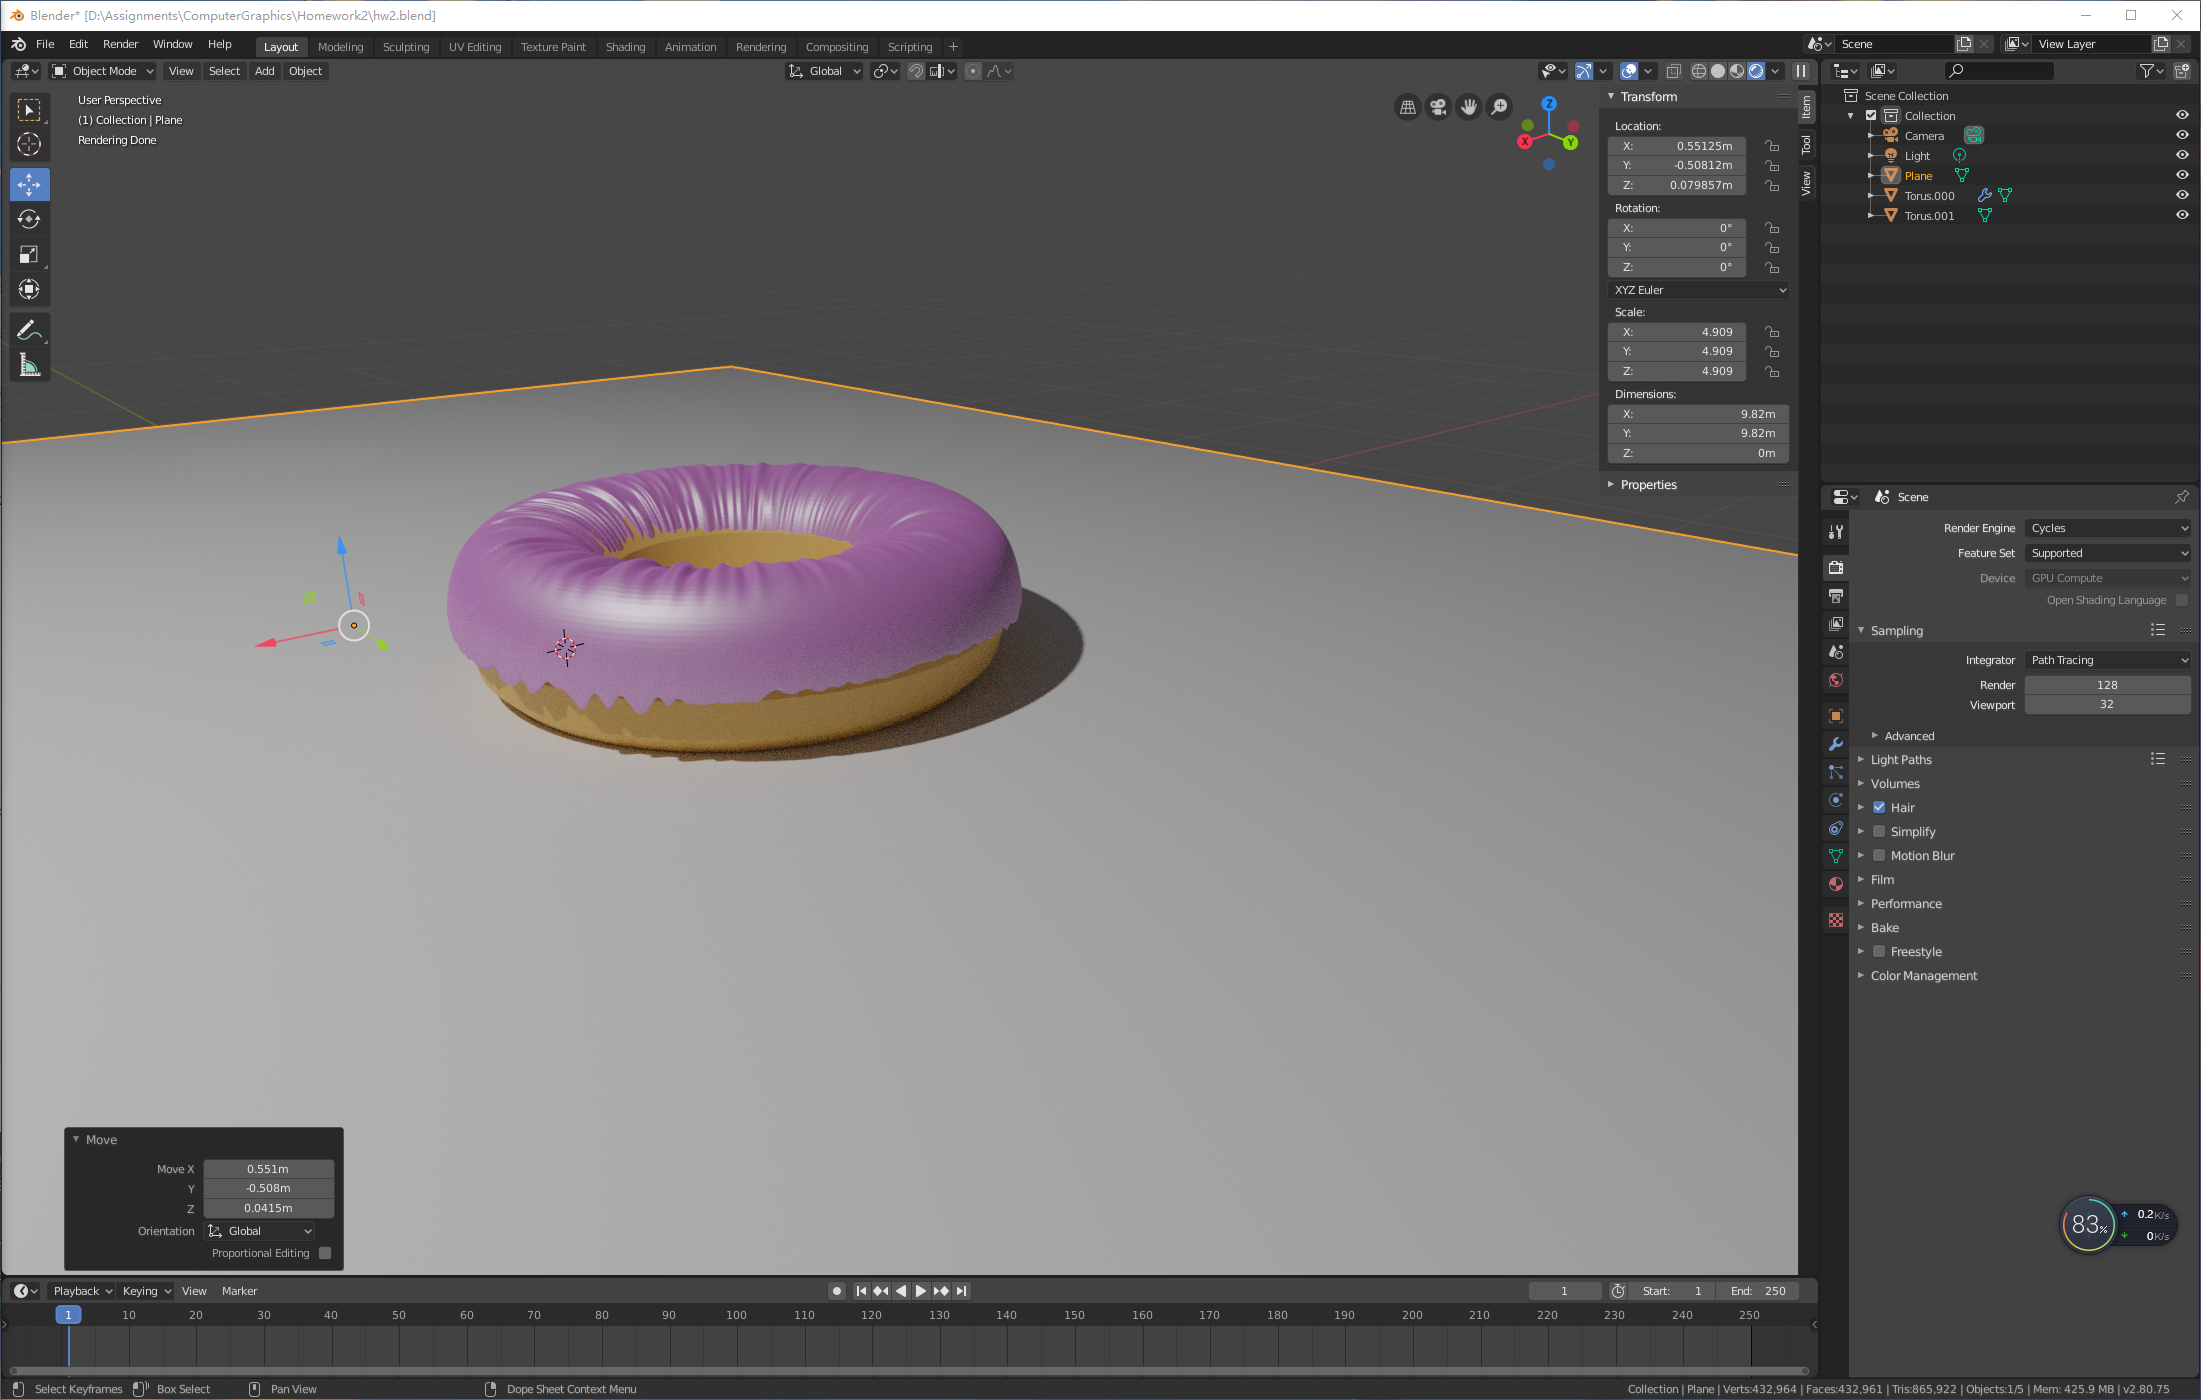
\includegraphics[width=\linewidth]{fig/v4-1.png}
\end{figure}
\begin{figure}[H]
\centering
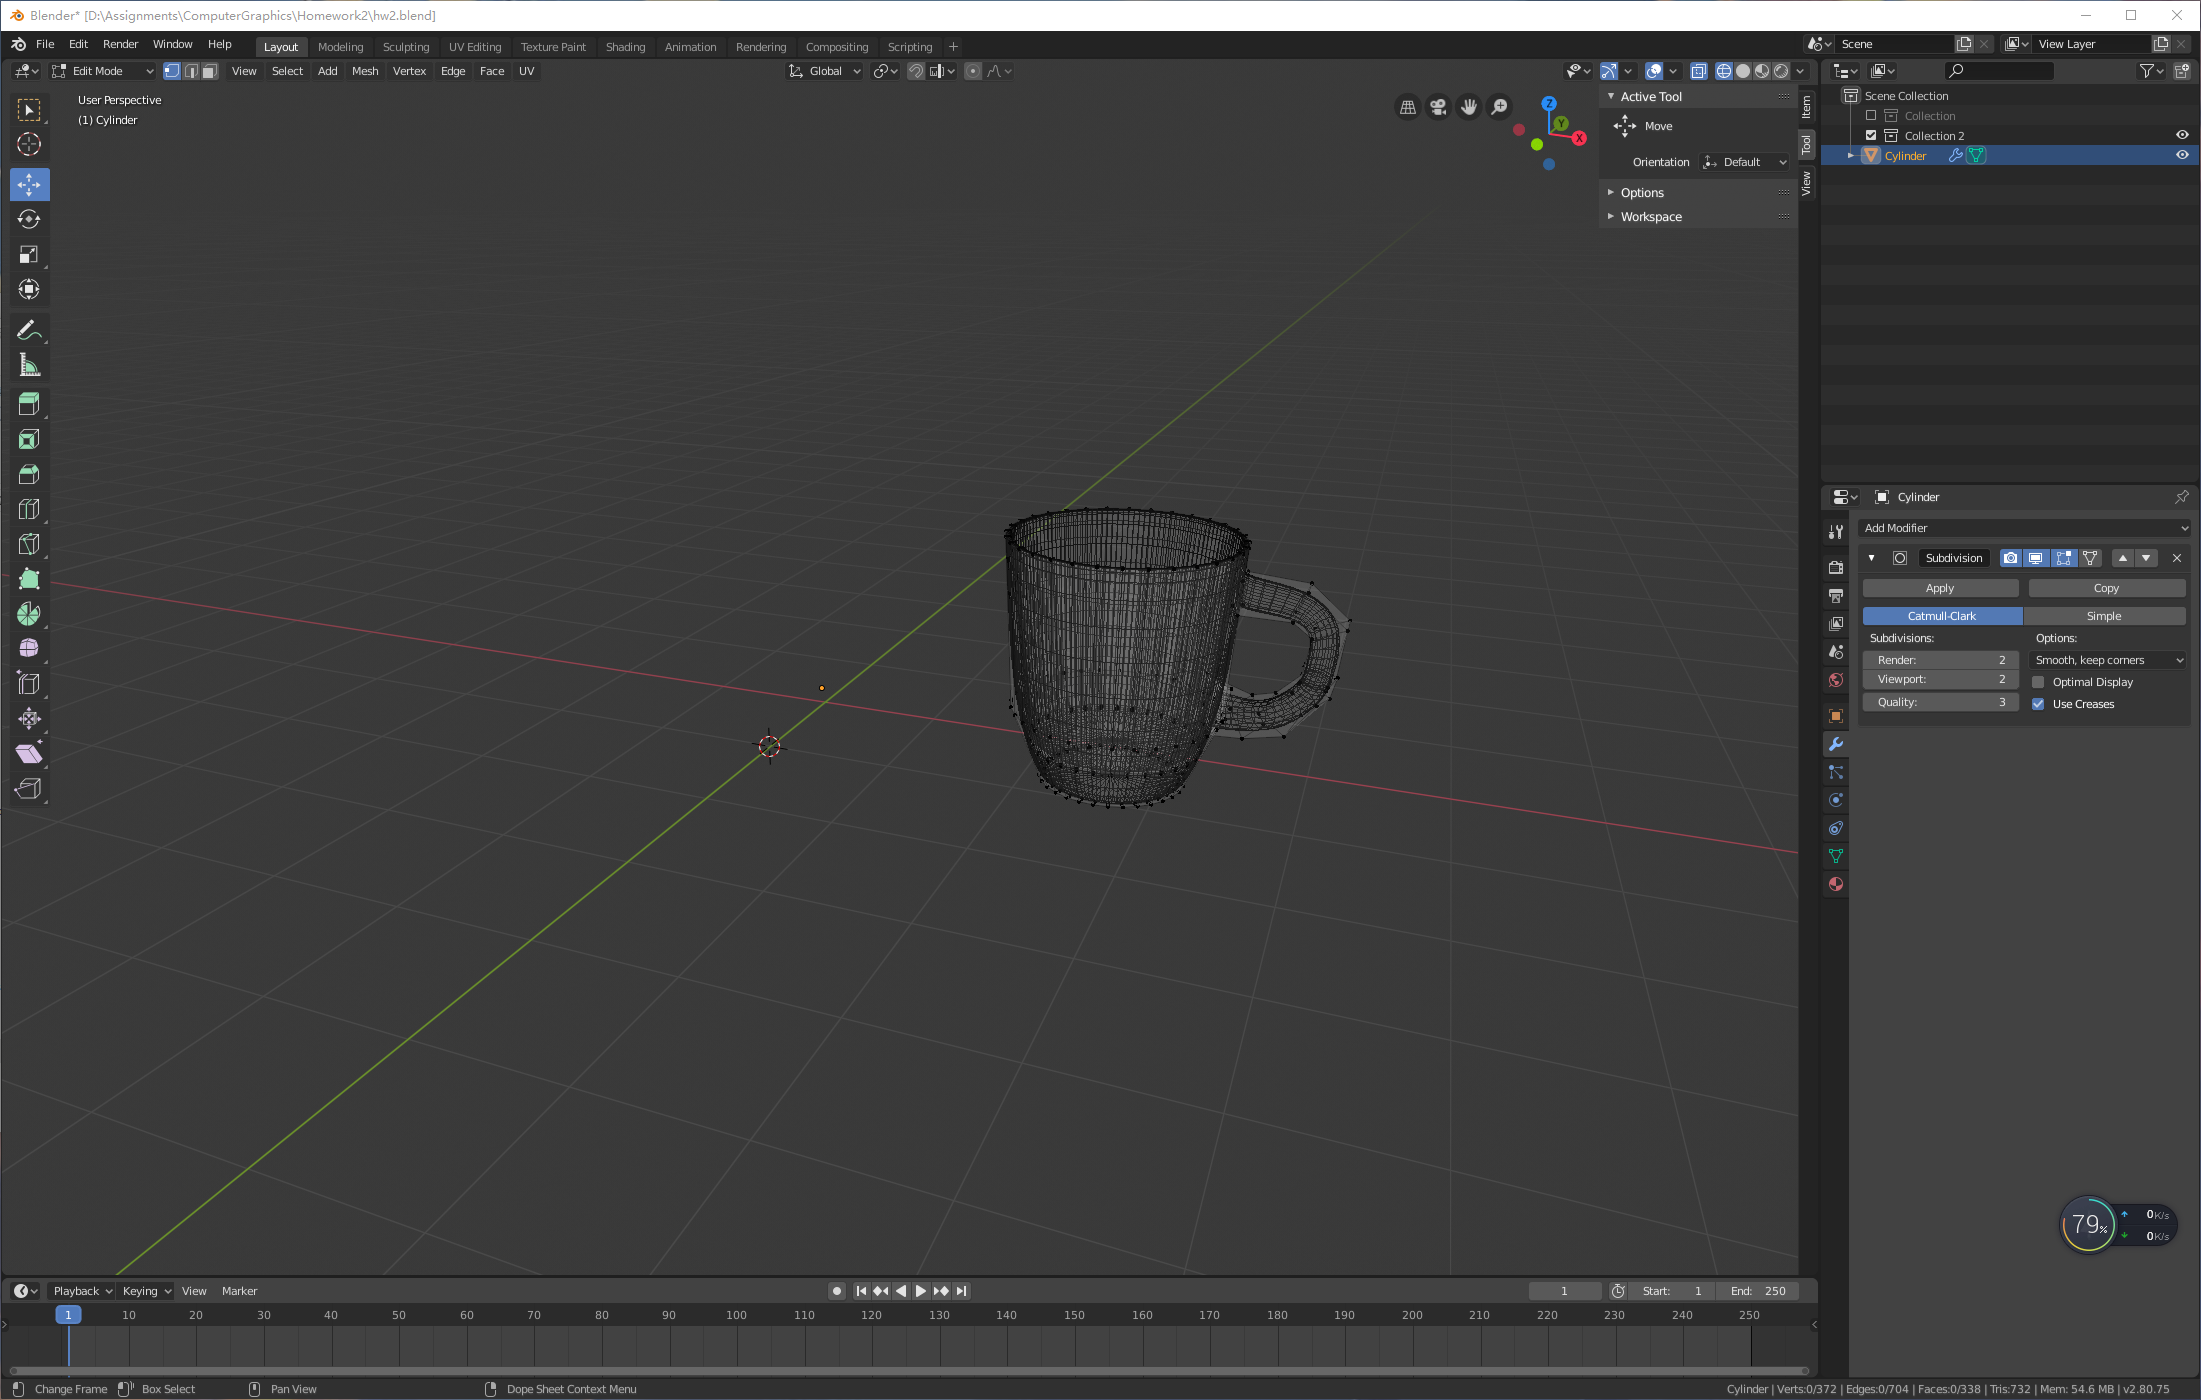
\includegraphics[width=\linewidth]{fig/v5.png}
\end{figure}
\begin{figure}[H]
\centering
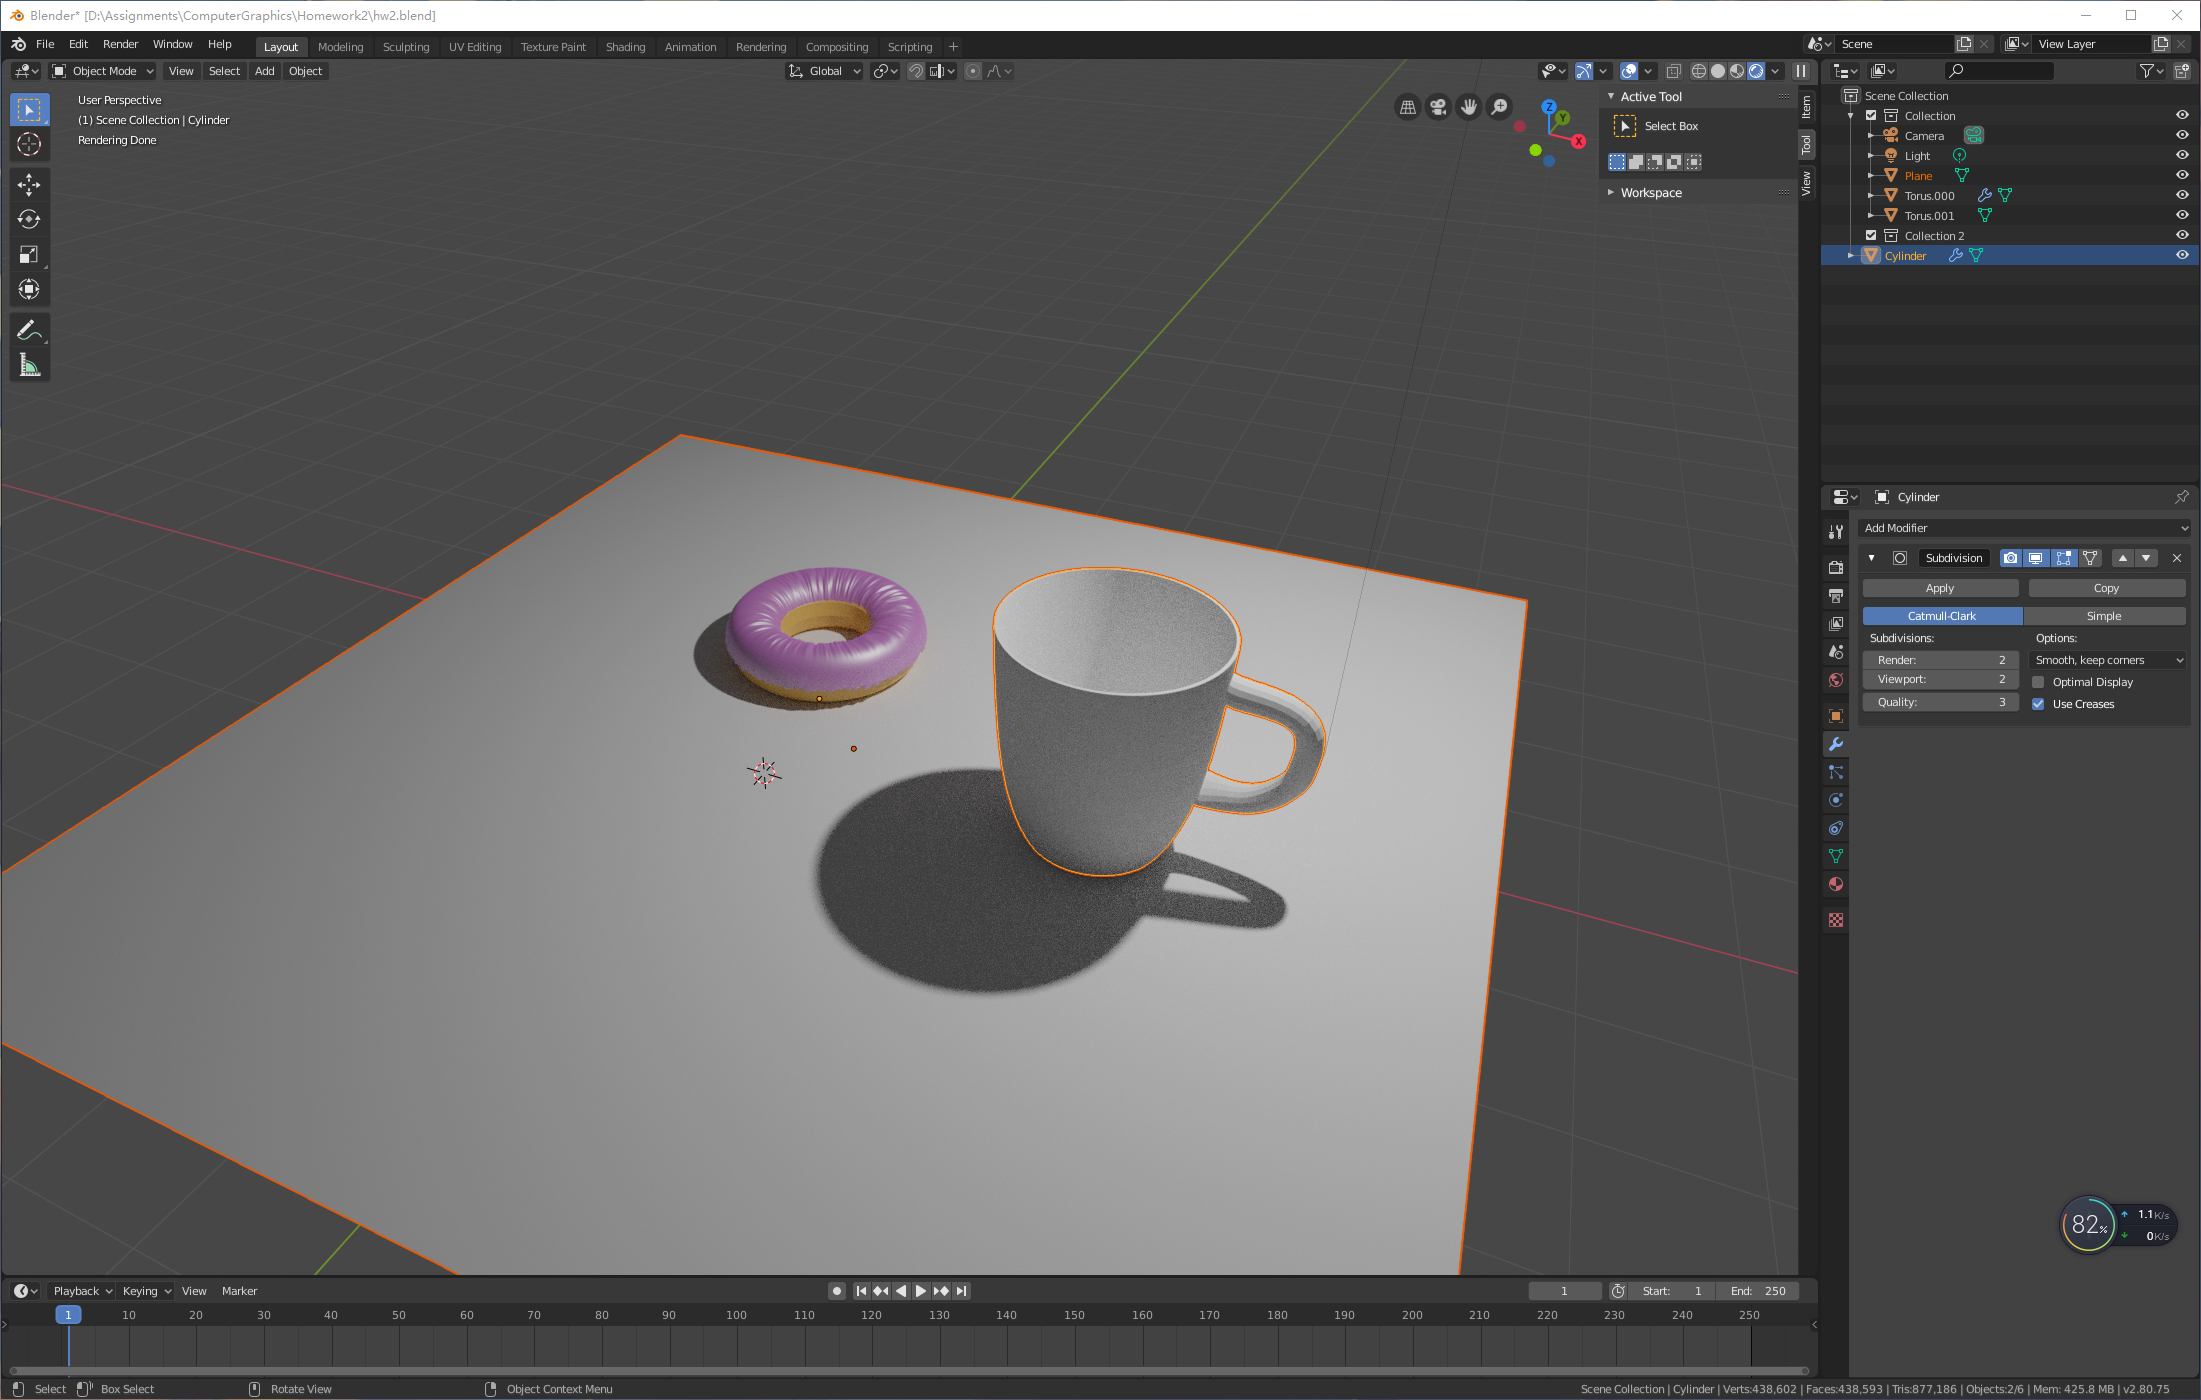
\includegraphics[width=\linewidth]{fig/v5-2.png}
\end{figure}
\begin{figure}[H]
\centering
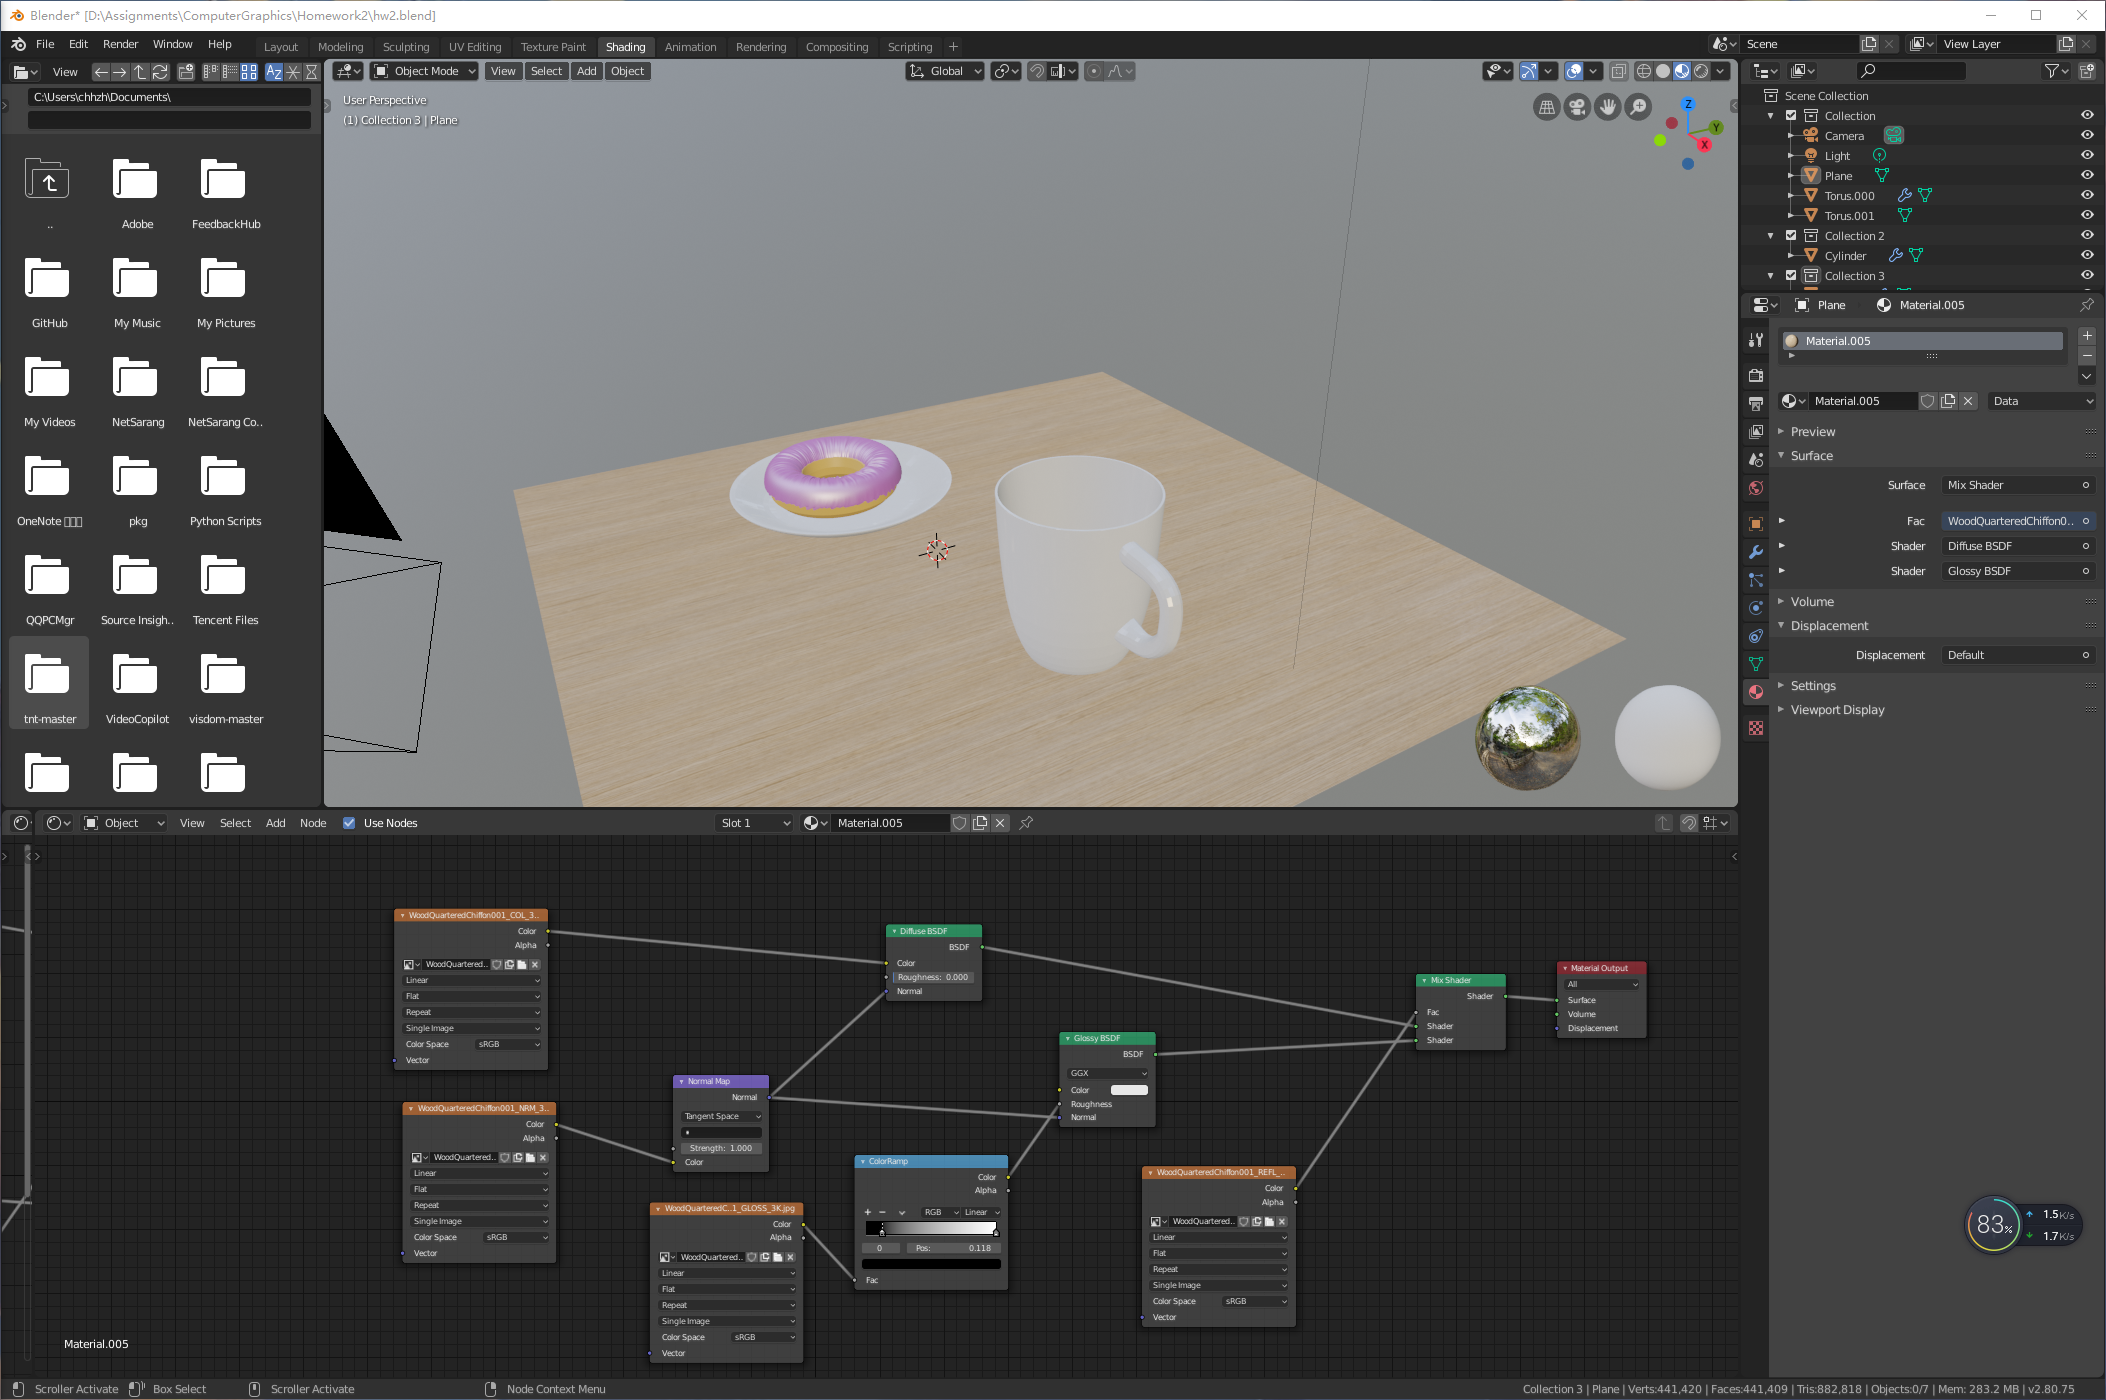
\includegraphics[width=\linewidth]{fig/v6.png}
\end{figure}
\begin{figure}[H]
\centering
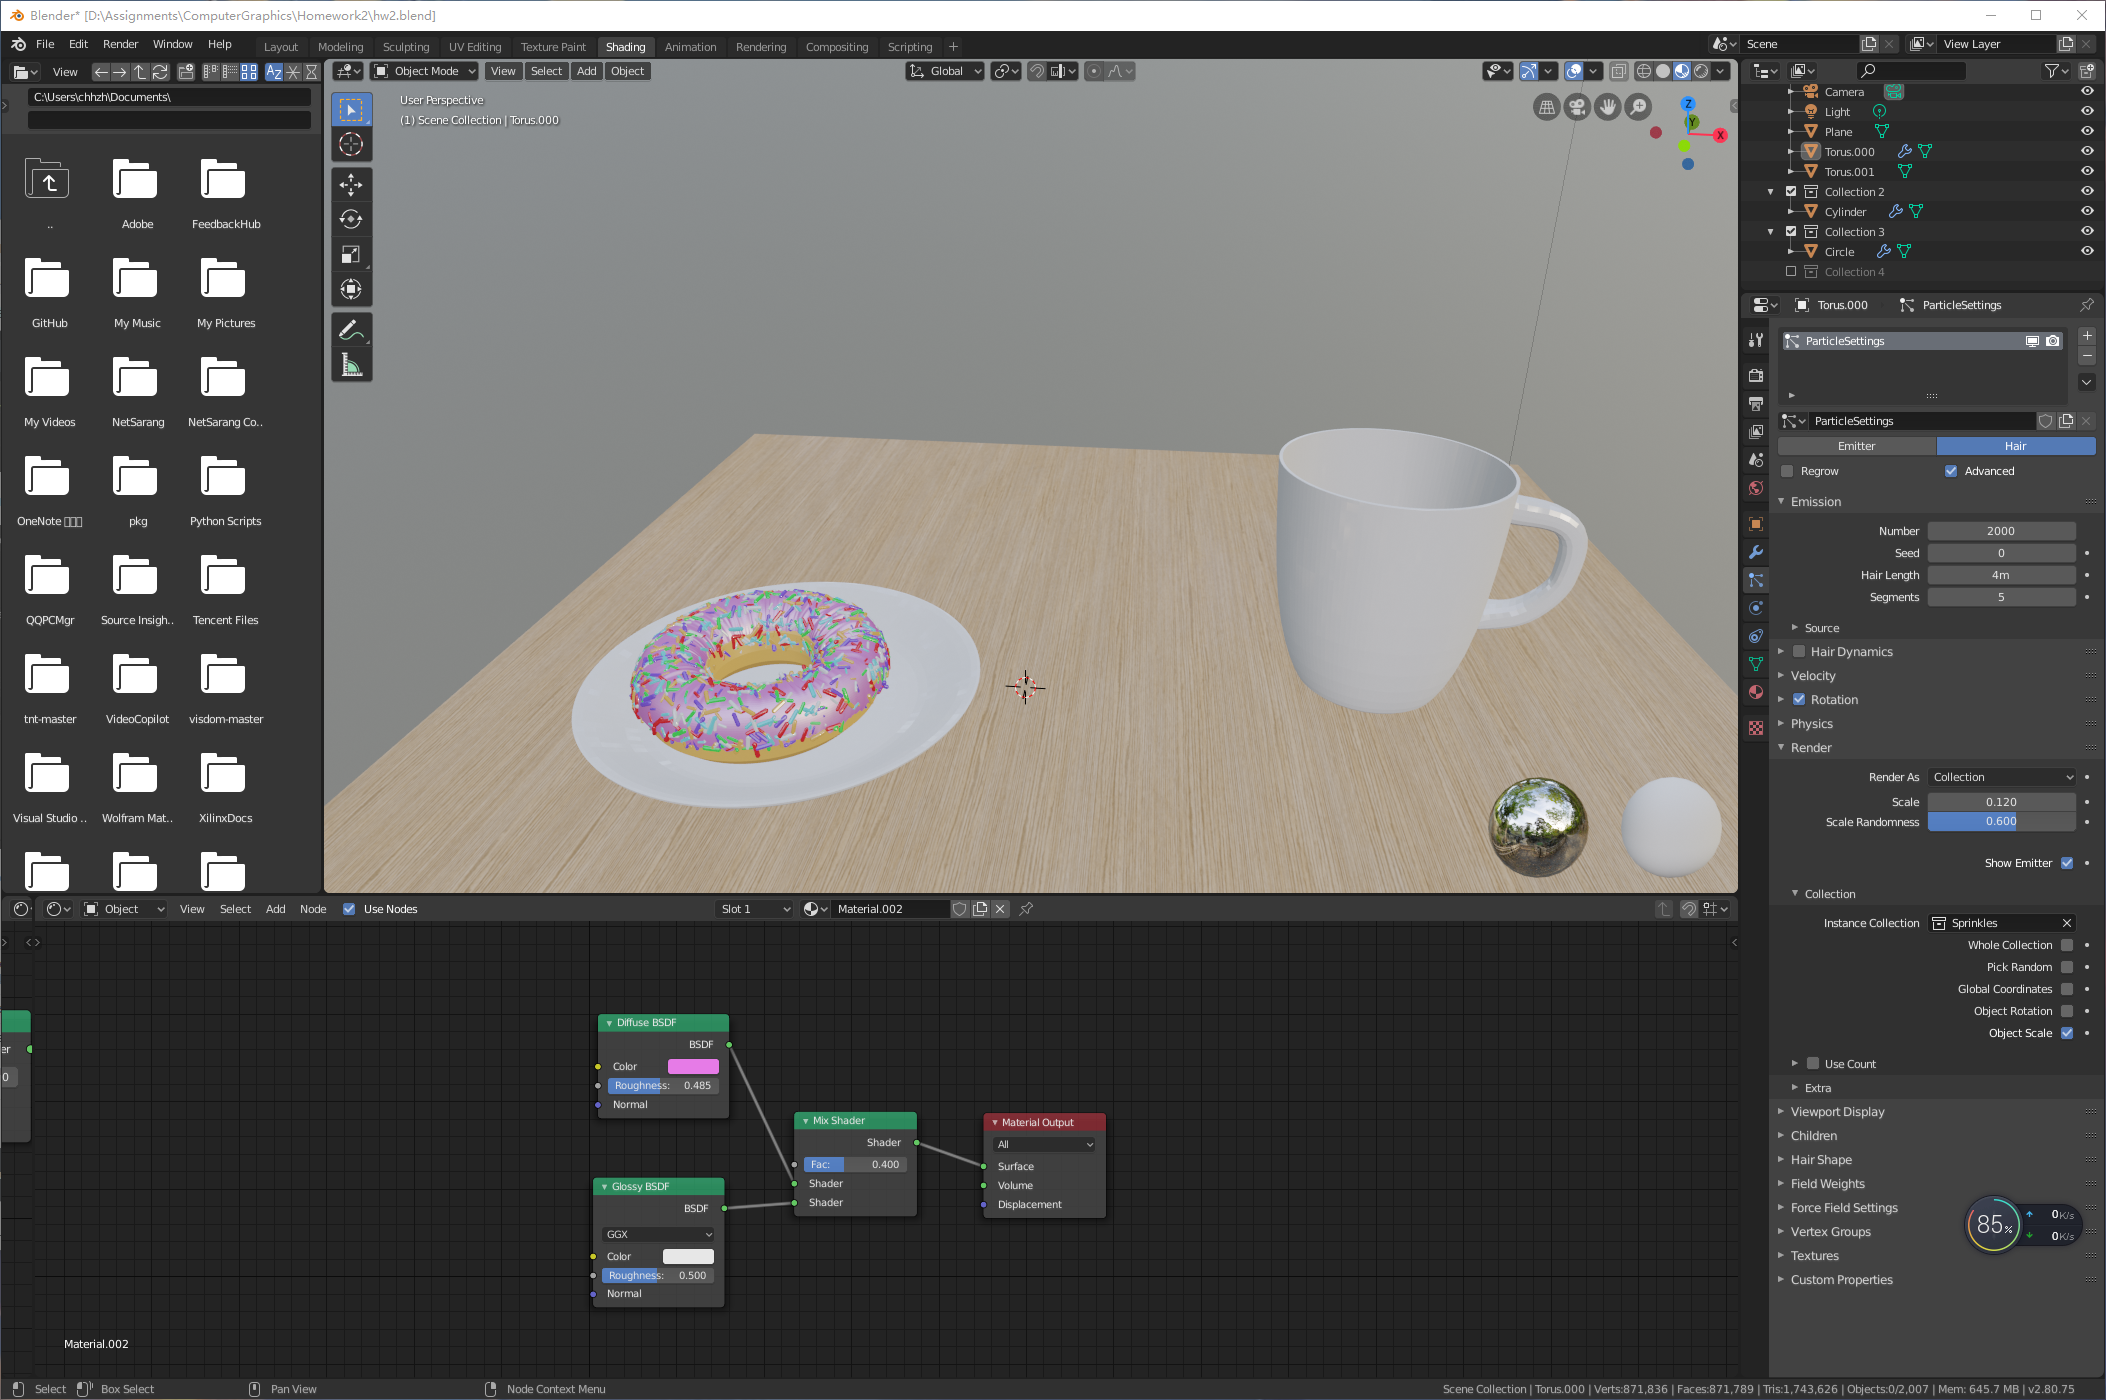
\includegraphics[width=\linewidth]{fig/v7.png}
\end{figure}
\begin{figure}[H]
\centering
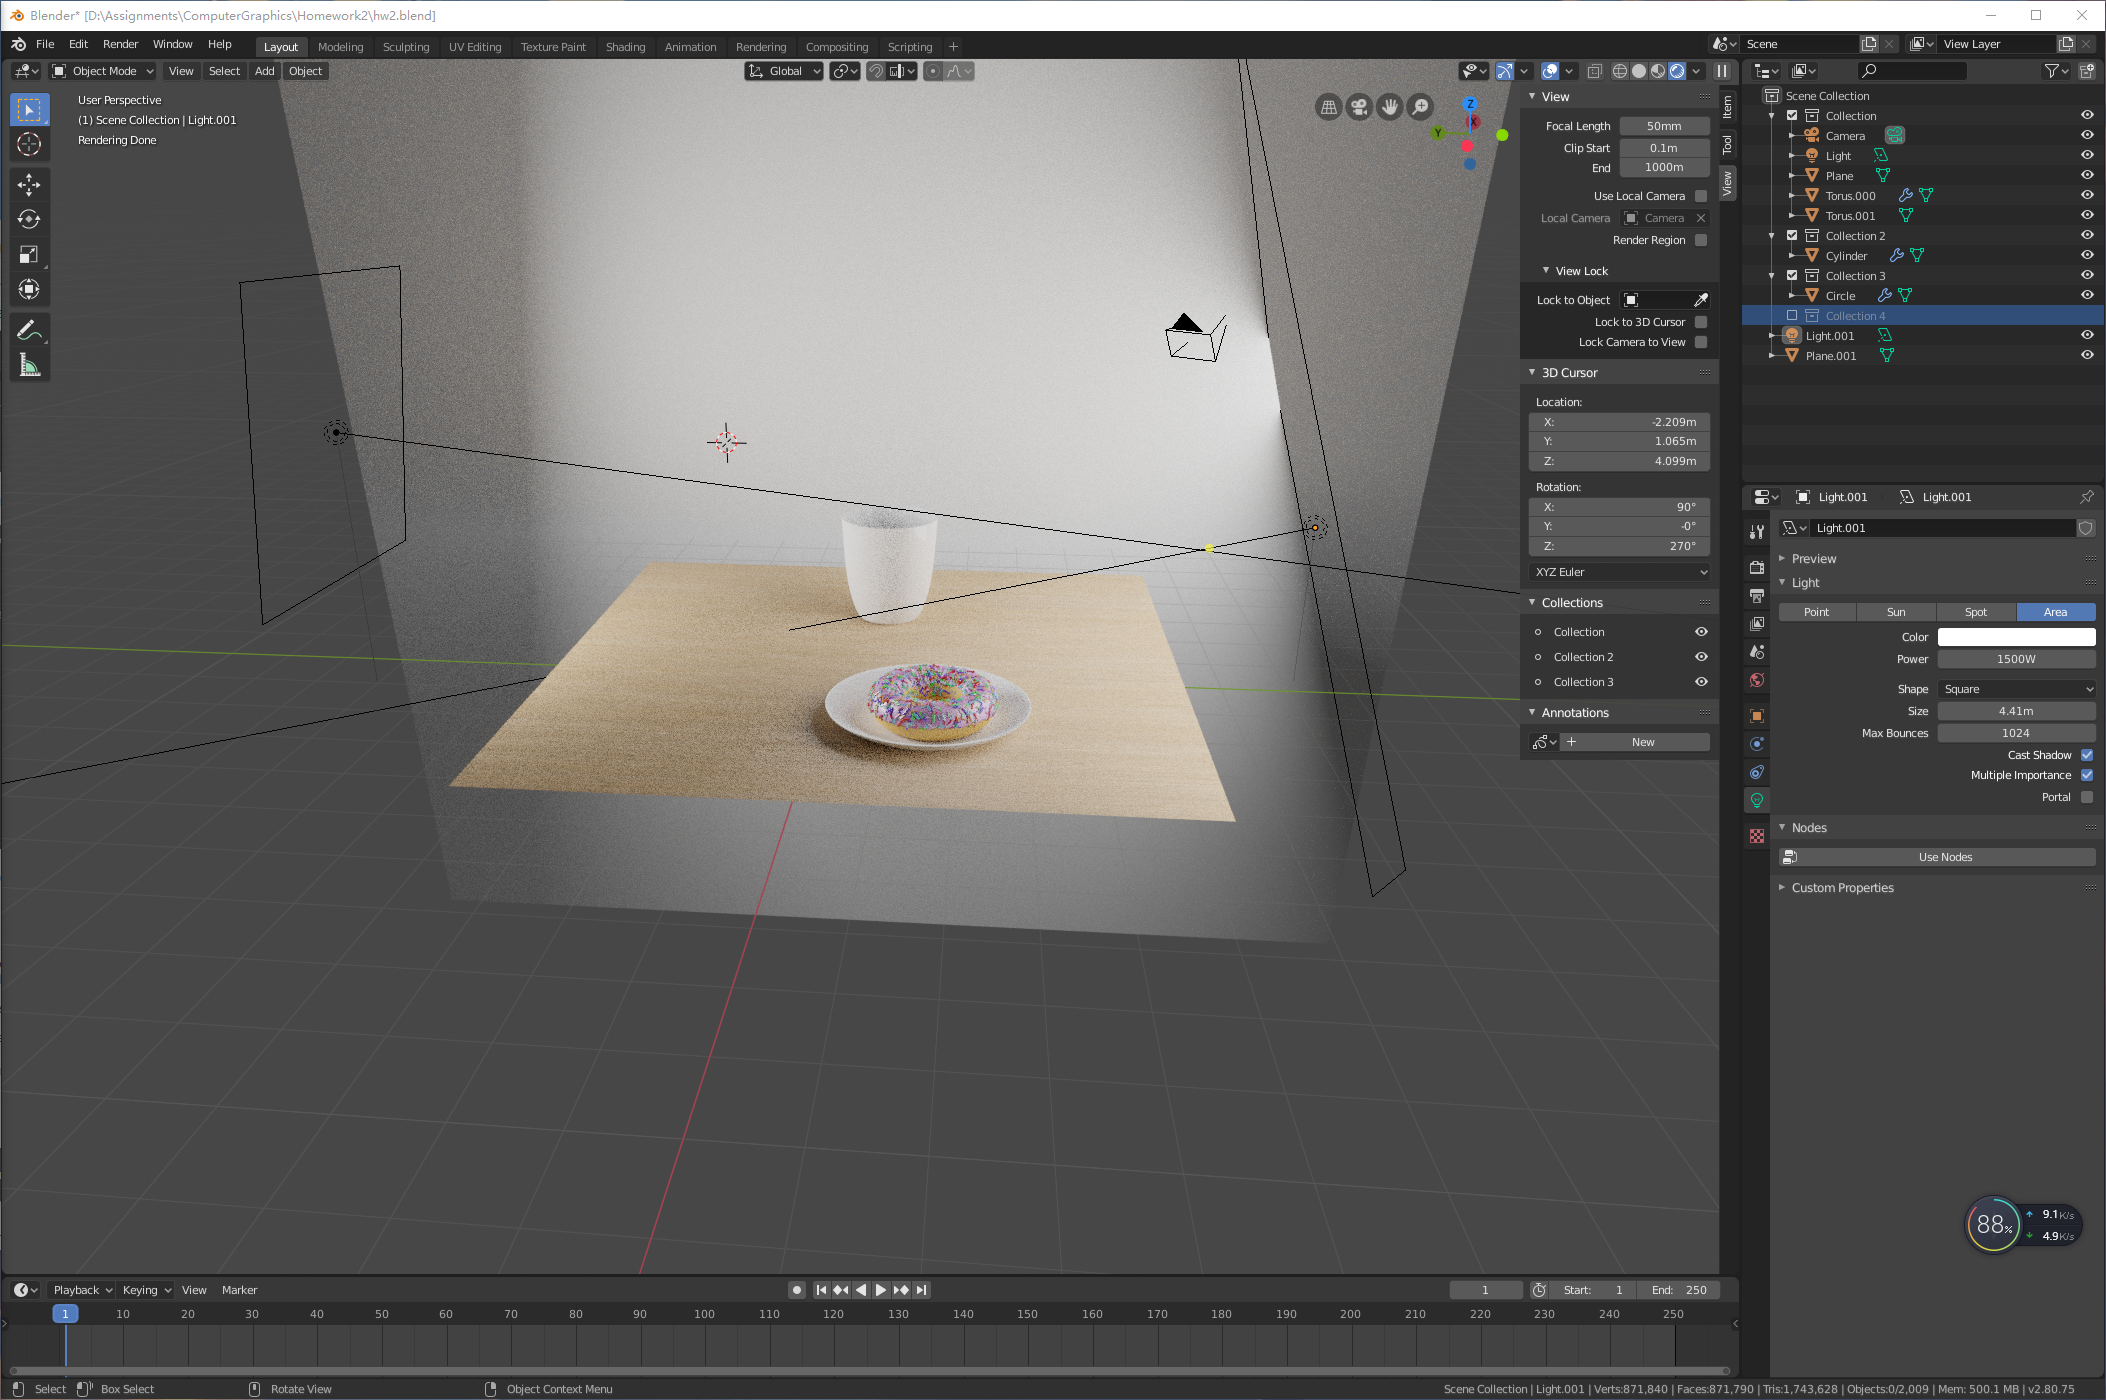
\includegraphics[width=\linewidth]{fig/v8.png}
\end{figure}
\begin{figure}[H]
\centering
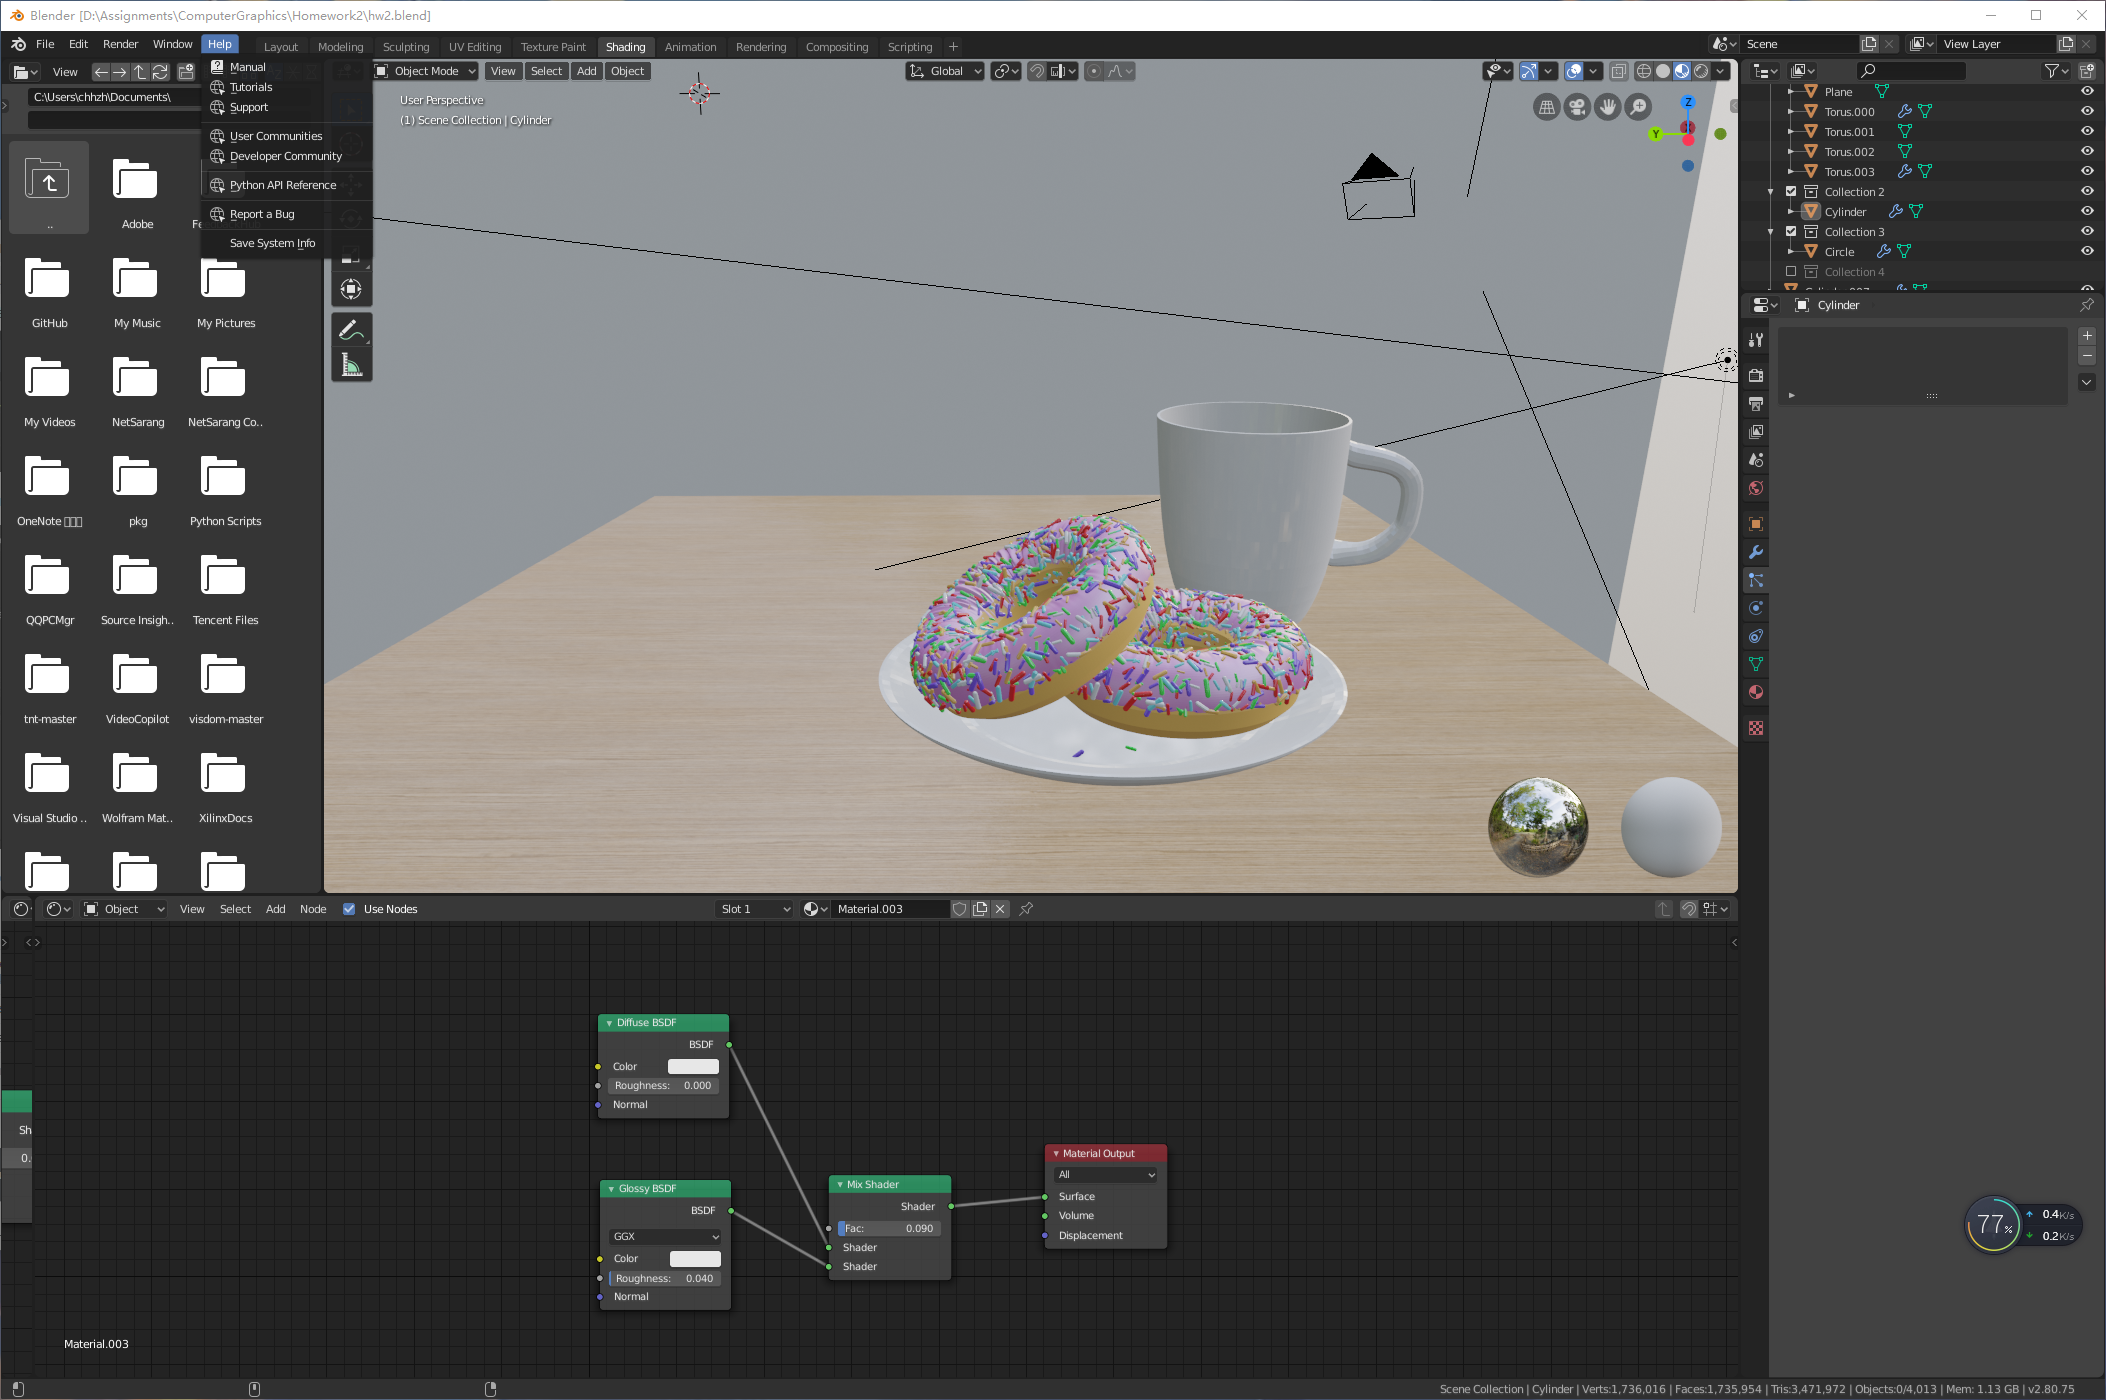
\includegraphics[width=\linewidth]{fig/v9.png}
\end{figure}

\end{document}

% 参考课程邮箱中主题为“Blender Beginner Tutorial” 的邮件附件视频, 学习使用 Blender 软件进行三维
% 建模和渲染, 并对 Graphical Rendering Pipeline 的原理进行理解。
% 视频也可以参考 bilibili 网站上的链接:
% https://www.bilibili.com/video/av14792640?from=search&seid=5961318134644031198
% https://www.bilibili.com/video/av29310333/?spm_id_from=333.788.videocard.1
% 链接内容与邮箱内容相同。 视频共 9 节, 总时长约 5 小时。
% 要求跟着视频教程, 从基本三维建模开始, 到实现对模型的渲染输出。 所得结果与视频教程中的结果
% 近似即可, 不要求完全一致。 也鼓励同学们发挥想象力, 做出更复杂的模型效果。
% 特别注意:
% 1. 由于软件版本与视频中所采用的版本不完全一致, 或视频演示不够清晰, 部分操作可能需要自行推
% 敲或通过别的方式替代。
% 2. 不允许下载网上现成的项目文件和模型, 建模需从零开始, 以掌握建模工具。
% 提交说明:
% 作业提交项目文件, 以及建模和渲染结果图像(若干张, 含中间结果图片), 发打包送到课程邮箱:
% cgcourse_homework@qq.com
% 若 2 天内没收到自动回复,请重新发邮件。 请于 9 月 15 日 24:00 前提交。
% 压缩包文件名格式如下:
% 班级 + 学号 + 姓名 + HW2
% 例: 17 计科+17000001+张三+HW2